\section{Simulation Model Description}

In this section the Arena model is described and explained. The model has been split into two models, firstly the management of the cashiers (main model) and secondly the management of the vehicles (submodel Pumps). The used variables, attributes and schedules will be described as well.

\subsection{Cashier management}
A screenshot of the complete cashier management model can be found in figure \ref{fig:model-cashier} in appendix \ref{app:modeldescription}.

This part of the model handles the checkouts and cashiers who work at them. It creates checkouts and assigns numbers to those (between 1 and 5, for the five checkout counters). A checkout is released just before a shift ends, so that it becomes available for an employee starting the shift after the current cashier, and so the new cashier can take over this checkout. When a checkout is released, an OnChange is triggered which puts it in the queue for seizing a cashier again. The creation of checkouts and assigning numbers can be seen in figure \ref{fig:createcheckouts}

\begin{figure}[h!]
	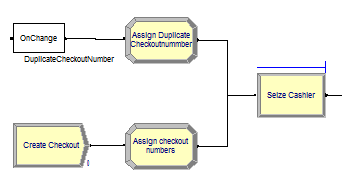
\includegraphics[scale=1]{images/model-description/checkout-creation.PNG}
	\caption{Modeling of the creation of checkouts.}
	\label{fig:createcheckouts}
\end{figure}

Then those checkouts seize a cashier (if available). If there are more than 5 cashiers active at the time, which can happen due to the checkout being released just before a shift ends and being seized by another cashier, the checkout is held at another queue called "Active Cashiers smaller than 5?". If this is not the case the checkout opens the lanes belonging to it. This part of the model can be seen in figure \ref{fig:seizeandopen}

\begin{figure}[h!]
	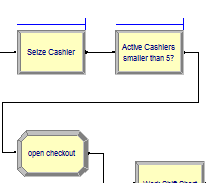
\includegraphics[scale=1]{images/model-description/seize-and-open.PNG}
	\caption{Modeling of the cashier seizing and checkout opening.}
	\label{fig:seizeandopen}
\end{figure}

After that the checkout has to wait for the cashier to finish his/her shift. This process can be seen in figure \ref{fig:workshift}. In the process, we first check whether it's a 2 hour or a 4 hour shift. The 2 hour shift only occurs when a cashier starts working at 10 p.m. and thus finishes his shift at 2 a.m. the next day. So he actually works a 4 hour shift, but for the current day, he only works from midnight until 2 a.m.
Apart from this exception, the delay is also 5 minutes short of these 2 or 4 hours. After this too short delay, the checkout is released ("Trigger OnChange") and the remaining 5 minutes delay are invoked.
When the cashier is completely done with his regular shift we decrease the number of active cashiers so the possibly stuck checkout can be let through the "Active Cashiers smaller than 5?" state we saw before.

\begin{figure}[]
	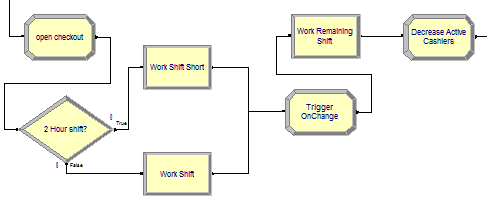
\includegraphics[scale=1]{images/model-description/work-shift.PNG}
	\caption{Modeling of the delay for the cashier working his/her shift.}
	\label{fig:workshift}
\end{figure}

After the regular shift, we have to determine what will happen to the lane and cashier. Does he close the lanes and continue working at the checkout? Or does another cashier take over and can he go over to restocking the supplies? This is checked in the blocks displayed in figure \ref{fig:determinetakeover}. As you can see, the check whether someone takes over is split into two checks. This is due to a technicality issue: when checking whether there is a new cashier that takes over the checkout, we check whether the checkout is taken again after the current cashier seized it (which can happen due to releasing the checkout 5 minutes before the end of the shift). This would mean the checkout would be taken over. In order to check this, we store the time each checkout is last seized (this is done in the "open checkout" block in figure \ref{fig:seizeandopen}) and then see if this was later than 3.5 hours ago. But this would not work if we were just starting out the day, e.g. between shift 12 and 1 and shift 1 and 2. Therefor we added another decide block which checks the time.
Then, the pump stays open module can check whether the checkout has been seized again and based on that decide what happens: the lane closes and the cashier stays, or the lane stays open and the cashier can start restocking.

\begin{figure}[]
	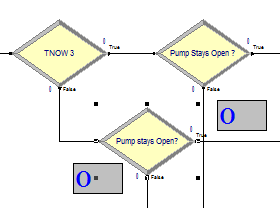
\includegraphics[scale=1]{images/model-description/determine-takeover.PNG}
	\caption{Modeling of the check whether a checkout is taken over.}
	\label{fig:determinetakeover}
\end{figure}

The last part of the cashier management is rather straightforward (figure \ref{closerestockandrelease}): based on the previous decision, the checkout is closed after which the cashier works until the lane and checkout queue are both empty after which he restocks the supplies if less than 10 minutes have passed since the checkout closing (which is calculated by setting a variable to the current time upon closing and comparing it to current time after the queue is emptied). Or the checkout does not close and the cashier immediately restocks the supplies.
After this the cashier is released and the checkout entity disposed of.

\begin{figure}[]
	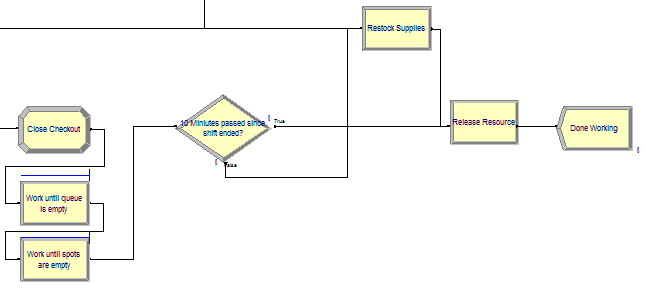
\includegraphics[scale=1]{images/model-description/close-restock-release.PNG}
	\caption{Modeling of the check whether a checkout is taken over.}
	\label{fig:closerestockandrelease}
\end{figure}

